\documentclass{article}
% Title of the paper:
\newcommand{\hemaClassTitle}{\hemaClass{}: Online one-by-one normalization and classification of hematological malignacies}

% Load packages
\usepackage{fullpage} % Larger margins
\usepackage{amssymb,amsmath}
\usepackage{authblk}  % For author affiliations
\usepackage[hypertexnames=false]{hyperref} % For urls and hyperlinks
\usepackage{graphicx}
\usepackage[numbers,sort]{natbib}
\usepackage{cite} % Make references as [1-4], not [1,2,3,4]

% To do notes
\usepackage[
%  disable, %turn off todonotes
  colorinlistoftodos, %enable a coloured square in the list of todos
  textwidth=2cm, %set the width of the todonotes
  textsize=scriptsize, %size of the text in the todonotes
  ]{todonotes}

% Macros
\newcommand{\hemaClass}{\href{http://hemaClass.org}{\texttt{hemaClass.org}}}
\newcommand{\R}{\textsf{R}}
\newcommand{\pkg}[1]{\textbf{#1}}

\DeclareMathOperator*{\median}{median}
\DeclareMathOperator*{\std}{std}

% Hypenation
\hyphenation{Chemo-resistance}



\begin{document}

\begin{center}
{\huge SUPPLEMENTARY MATERIAL - RLE}\bigskip \\
\end{center}

\section{Model control of reference based RMA normalization}
Given the large difference in misclassifications  between one-by-one and reference normalized samples, we would like to be able to distinguish between the two in a setting where we are unsure how closely the RMA reference resembles the samples.

\subsection{Relative Log Expression}
The relative log expression (RLE)	is a quality measure for microarrays introduced by \citet{Bolstad2004b}. If we define $\hat{\theta}_{ij}$ as the estimated log expression for probe $i$ on array $j$ following RMA normalization, the RLE is given by:
\[
\textrm{RLE}(\hat{\theta}_{ij}) = \hat{\theta}_{ij} - \textrm{median}_j(\hat{\theta}_{ij})
\]
i.e. the difference between the expression on a given array and the median expression in the cohort. A non-zero median RLE across probes for an array thus indicates differences in the number of up- and downregulated genes, while a large interquartile range (IQR) indicates that most genes on a given array are differentially expressed \citep{McCall2011}. Extreme values of these measures may be used to identify arrays with low-quality data. We propose that it may also be used to evaluate how well a sample resembles a given RMA reference following normalization (how well it has been normalized), by substituting the cohort median with the RMA reference median.

\section{Results}
For each of the five datasets used in the current study a random subset of 30 samples were extracted and set as a user reference. The remaining samples for each dataset where then RMA normalized as a cohort, against the randomly selected user reference (reference based) or against the four other datasets (one-by-one). RLE values were calculated in all six scenarios and summarized as the median and IQR for each sample. These values are shown in panel A and B in \cref{fig:chep_rle} to \cref{fig:mdfci_rle}. We find that the RLE values in the user reference scenarios more closely resemble the values calculated from cohort normalization than the values from one-by-one normalization. Furthermore differences between reference-based and on-by-one are more pronounced for the IQR of RLE than for the median. ROC curves showing the ability of the RLE median or IQR to distinguish between a user reference and a one-by-one reference were calculated and plotted using the pROC package version 1.8 \citep{Robin2011} in \R, as shown in panels C and D in \cref{fig:chep_rle} to \cref{fig:mdfci_rle}. The area under the curve (AUC) for the ROC curves confirm the superiority of the RLE IQR for distinguishing between a "correct" user reference and a "wrong" reference, i.e. in most cases we observe a higher AUC when using the IQR instead of the median RLE.\\\\
Using Youden's index, which maximizes the sum of sensitivity and specificity, we calculated the optimal threshold for each ROC curve based on the RLE IQR as shown in table \ref{rleTable}. Calculating the median RLE IQR across all datasets and one-by-one RMA references gives a value of 0.615. By rounding of we set a conservative threshold of 0.6 for reference normalized samples, i.e. if the RLE IQR exceeds this value we advise not to include the sample in subsequent classifications. This does not remove all one-by-one normalized samples, but in most cases it prevents the user from getting poor classifications resulting from biased RMA normalization.

\begin{figure}
	\begin{center}
		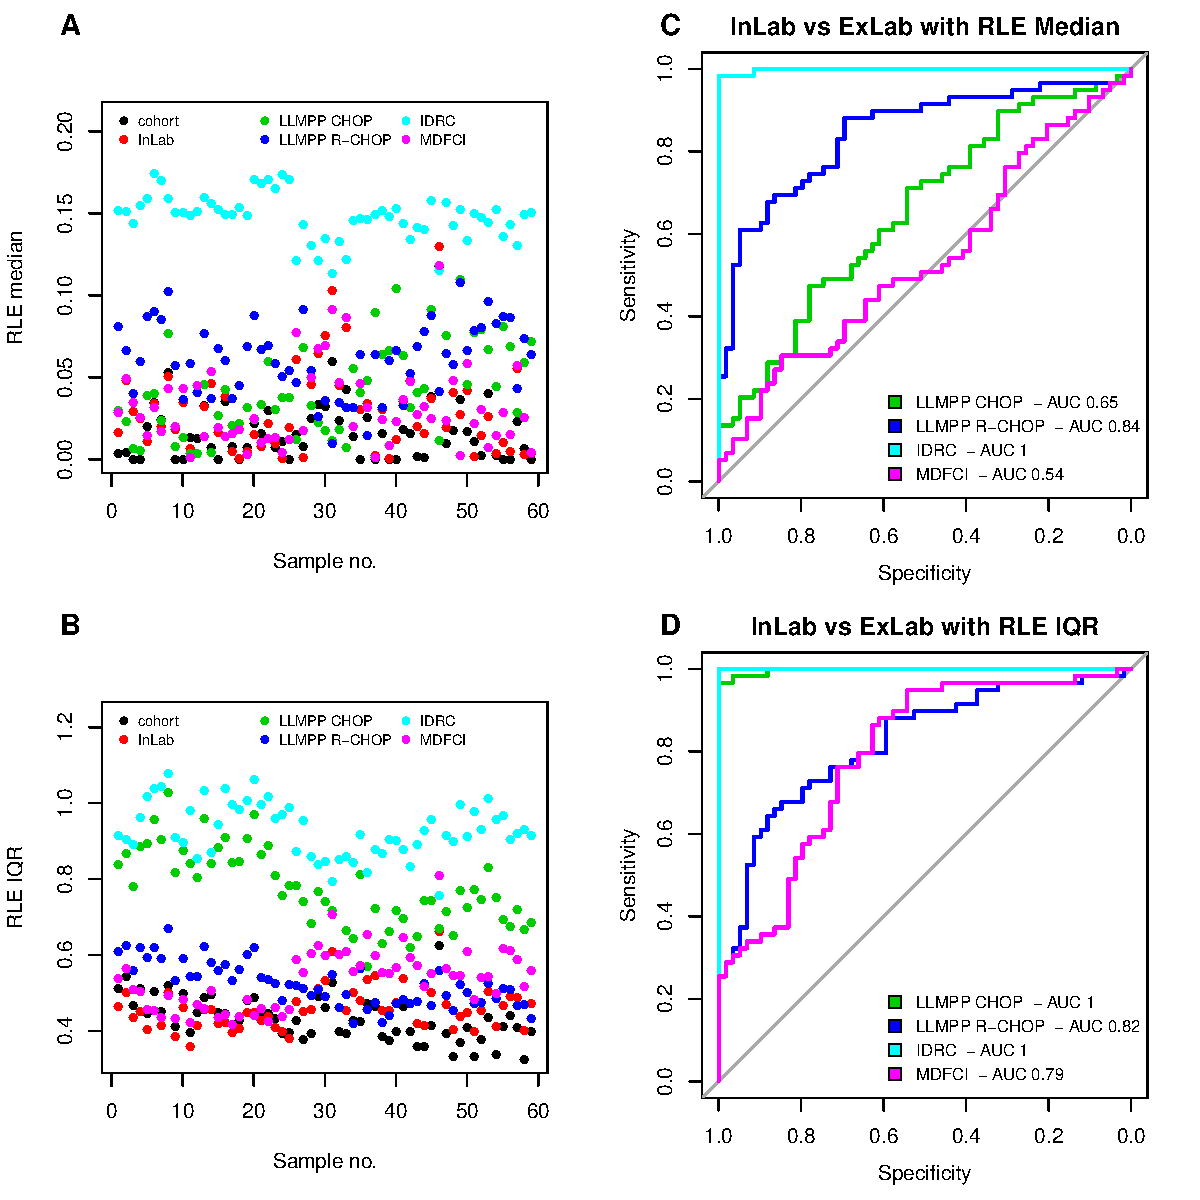
\includegraphics[width=0.8\textwidth]{figures/chep_rle.pdf}
	\end{center}
	\caption{Median and IQR RLE values for different RMA normalizations of the CHEPRETRO dataset and ROC curves}
	\label{fig:chep_rle}
\end{figure}

\begin{figure}
	\begin{center}
		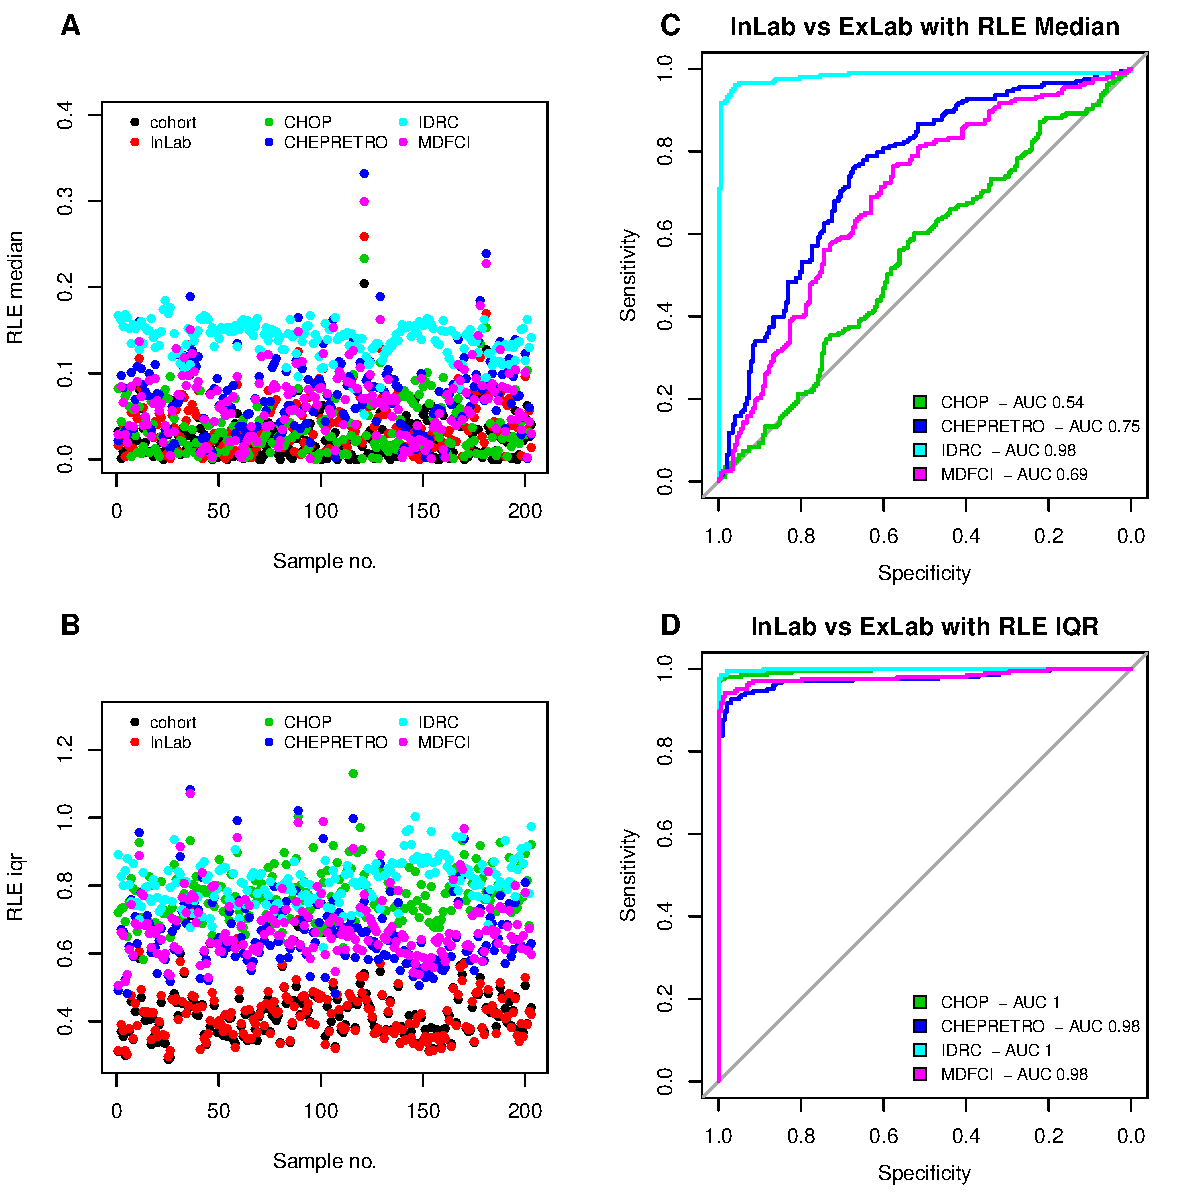
\includegraphics[width=0.8\textwidth]{figures/RCHOP_rle.pdf}
	\end{center}
	\caption{Median and IQR RLE values for different RMA normalizations of the RCHOP dataset and ROC curves}
	\label{fig:rchop_rle}
\end{figure}

\begin{figure}
	\begin{center}
		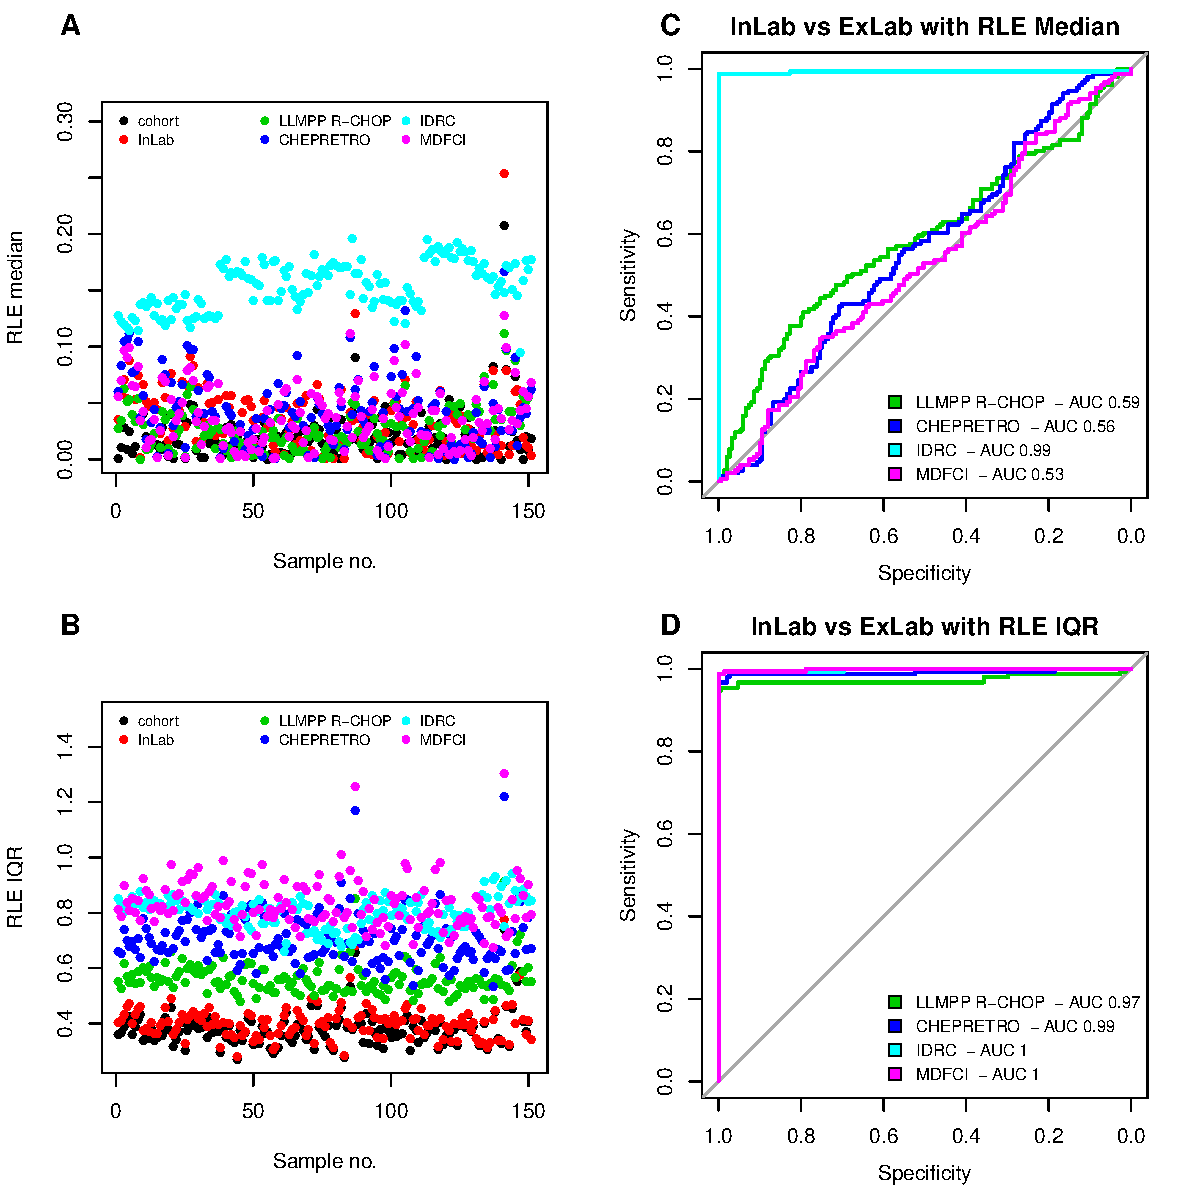
\includegraphics[width=0.8\textwidth]{figures/CHOP_rle.pdf}
	\end{center}
	\caption{Median and IQR RLE values for different RMA normalizations of the CHOP dataset and ROC curves}
	\label{fig:chop_rle}
\end{figure}

\begin{figure}
	\begin{center}
		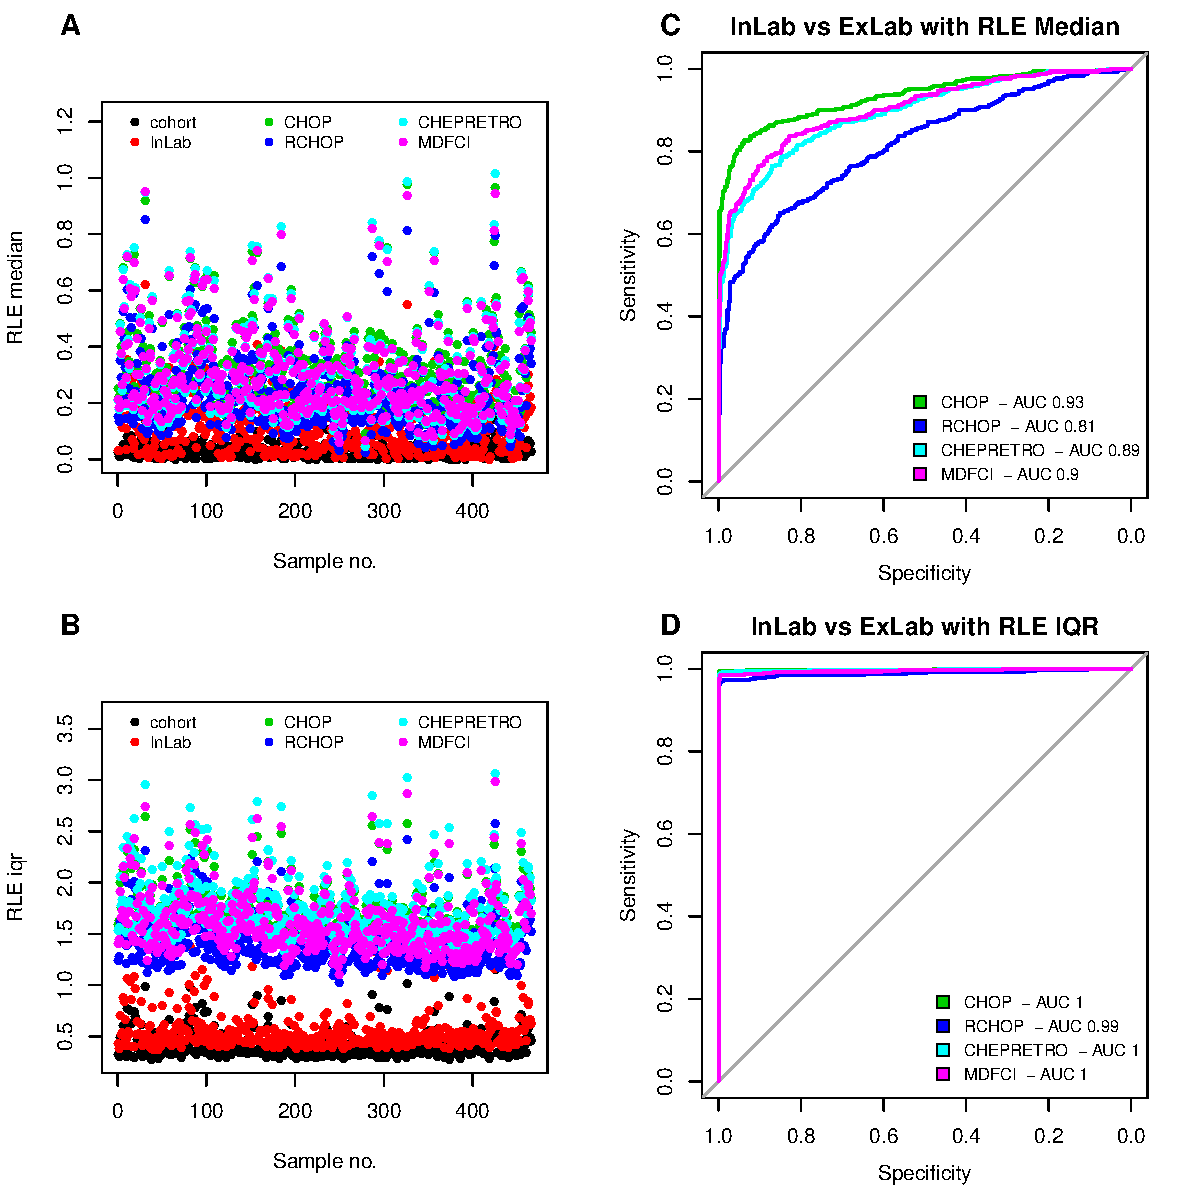
\includegraphics[width=0.8\textwidth]{figures/IDRC_rle.pdf}
	\end{center}
	\caption{Median and IQR RLE values for different RMA normalizations of the IDRC dataset and ROC curves}
	\label{fig:idrc_rle}
\end{figure}

\begin{figure}
	\begin{center}
		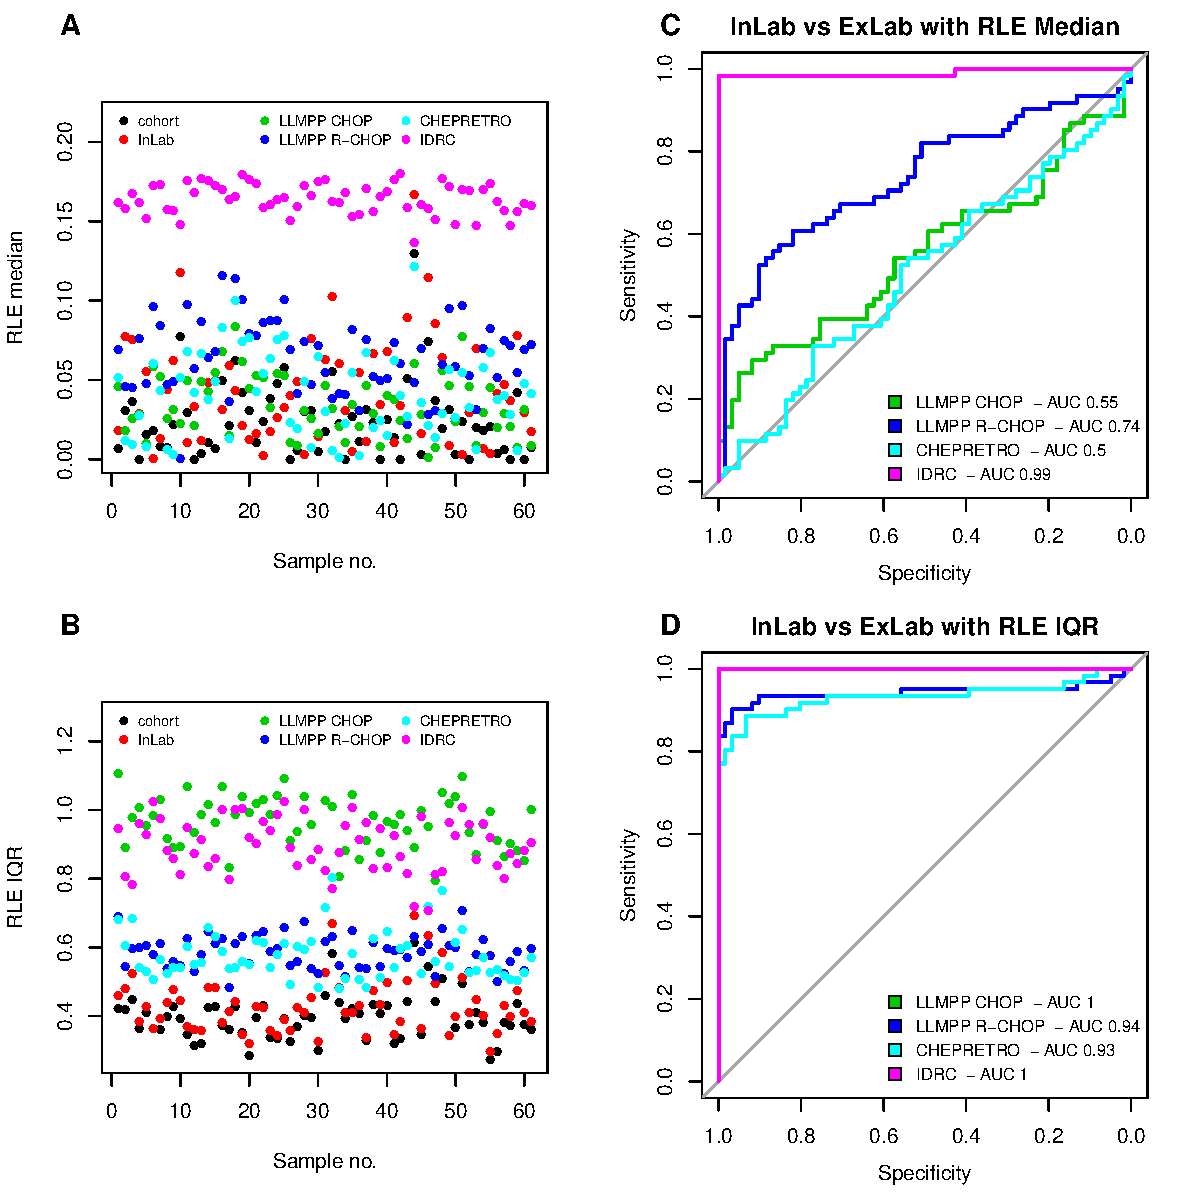
\includegraphics[width=0.8\textwidth]{figures/MDFCI_rle.pdf}
	\end{center}
	\caption{Median and IQR RLE values for different RMA normalizations of the MDFCI dataset and ROC curves}
	\label{fig:mdfci_rle}
\end{figure}


% latex table generated in R 3.3.1 by xtable 1.8-2 package
% Mon Aug 29 13:49:06 2016
\begin{table}[ht]
\centering
\begin{tabular}{llrrr}
  \hline
Dataset & RMA reference & Threshold & Sensitivity & Specificity \\ 
  \hline
CHEPRETRO & LLMPP CHOP & 0.56 & 0.97 & 1.00 \\ 
  CHEPRETRO & LLMPP R-CHOP & 0.47 & 0.68 & 0.85 \\ 
  CHEPRETRO & IDRC & 0.71 & 1.00 & 1.00 \\ 
  CHEPRETRO & MDFCI & 0.54 & 0.95 & 0.54 \\ 
  LLMPP R-CHOP & LLMPP CHOP & 0.61 & 0.98 & 1.00 \\ 
  LLMPP R-CHOP & CHEPRETRO & 0.52 & 0.93 & 0.97 \\ 
  LLMPP R-CHOP & IDRC & 0.68 & 0.99 & 1.00 \\ 
  LLMPP R-CHOP & MDFCI & 0.53 & 0.94 & 0.99 \\ 
  LLMPP CHOP & LLMPP R-CHOP & 0.48 & 0.95 & 0.99 \\ 
  LLMPP CHOP & CHEPRETRO & 0.51 & 0.97 & 1.00 \\ 
  LLMPP CHOP & IDRC & 0.62 & 0.99 & 1.00 \\ 
  LLMPP CHOP & MDFCI & 0.62 & 0.99 & 1.00 \\ 
  IDRC & LLMPP CHOP & 1.39 & 0.99 & 1.00 \\ 
  IDRC & LLMPP R-CHOP & 1.08 & 0.97 & 1.00 \\ 
  IDRC & CHEPRETRO & 1.32 & 0.99 & 1.00 \\ 
  IDRC & MDFCI & 1.19 & 0.98 & 1.00 \\ 
  MDFCI & LLMPP CHOP & 0.74 & 1.00 & 1.00 \\ 
  MDFCI & LLMPP R-CHOP & 0.51 & 0.90 & 0.97 \\ 
  MDFCI & CHEPRETRO & 0.50 & 0.89 & 0.93 \\ 
  MDFCI & IDRC & 0.70 & 1.00 & 1.00 \\ 
  Median & - & 0.62 & 0.97 & 1.00 \\ 
   \hline
\end{tabular}
\caption{Optimal thresholds for RLE IQR} 
\label{rleTable}
\end{table}


\bibliographystyle{plainnat}
\bibliography{references}
\end{document}
